\documentclass[tikz,border=10pt]{standalone}
\usetikzlibrary{arrows.meta}

\begin{document}
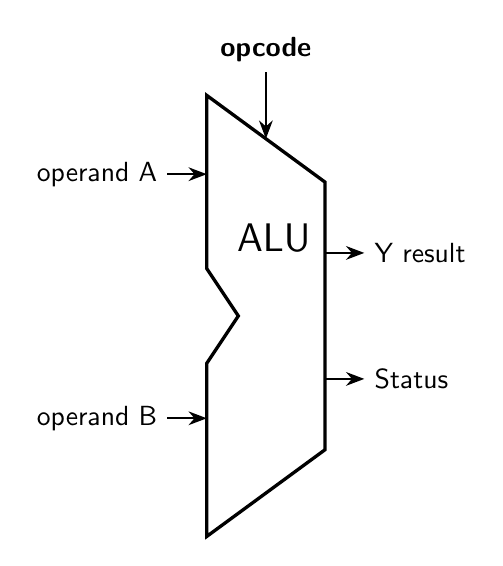
\begin{tikzpicture}[
    >=Stealth,
    font=\sffamily,
    line width=0.8pt
]

    % ALU Symbol Outline
    \draw[line width=1.2pt] 
        (0, 2.8) -- (1.5, 1.7) -- (1.5, -1.7) -- (0, -2.8) 
        -- (0, -0.6) -- (0.4, 0) -- (0, 0.6) -- cycle;

    % Label
    \node at (0.85, 1) {\Large ALU};

    % Left Inputs
    \draw[->] (-0.5, 1.8) node[left] {operand A} -- (0, 1.8);
    \draw[->] (-0.5, -1.3) node[left] {operand B} -- (0, -1.3);

    % Top Control Signal (ALU operation)
    \draw[<-,  thick] (0.75, 2.25) -- (0.75, 3.1) 
        node[above,  font=\sffamily\bfseries] {opcode};

    % Right Outputs
    \draw[->] (1.5, 0.8) -- (2.0, 0.8) node[right] {Y result};
    \draw[->] (1.5, -0.8) -- (2.0, -0.8) node[right] {Status};

\end{tikzpicture}
\end{document}